\documentclass[a4paper, 11pt]{article}

\setcounter{tocdepth}{3}
\setcounter{secnumdepth}{3}

\usepackage{comment} % enables the use of multi-line comments (\ifx \fi) 
\usepackage{lipsum} %This package just generates Lorem Ipsum filler text. 
\usepackage{fullpage} % changes the margin
\usepackage[utf8]{inputenc}
\usepackage{gensymb}
\usepackage{graphicx}
\usepackage{booktabs}% http://ctan.org/pkg/booktabs
\usepackage{makecell}
\usepackage{tabularx}
\usepackage[table]{xcolor}
\usepackage{array}
\usepackage{wrapfig}
\usepackage{subcaption}
\usepackage{csquotes}
\usepackage{lscape}
\usepackage{afterpage}
\usepackage{geometry}
\usepackage{listings}

\geometry{a4paper, margin=1in}
\renewcommand{\figurename}{Abb.}

\begin{document}
\title{Zusammenfassung Data Warehousing FS2018}
\author{Alex Neher}
\maketitle

\tableofcontents
\newpage

\graphicspath{{./Pictures/}}

\section{Die Notwendigkeit von Data Warehouses}
\subsection{Entscheidungsunterstützung (Skript S11)}
Data Warehouses sind keine neue Erfindung. Bereits in den 1960er Jahren wurden sogenannte \textbf{Managementsinformationssysteme} entwickelt. Diese MIS dienten dazu, Entscheidungsträgern alle benötigten Informationen zeitnah, fehlerfrei, flexibel, ergonomisch, effizient, effektiv und inspirativ zur Verfügung zu stellen. Diese Systeme treffen also nicht selbst Entscheidungen, sie \textbf{unterstützen} die Entscheidungsträger lediglich bei ihrer Entscheidung.

Es gibt vier Arten der Entscheidungsunterstützung:

\begin{description}
	\item [Modellbasiert:] z.B. Lineare Optimierung - Ein Mathematischer Ansatz basierend auf einem Modell $\Longrightarrow$ Abbildung der Realität
	\item [Wissensbasiert: ] z.B. Expertensysteme - Ansätze von Künstlicher Intelligenz
	\item [Datenbasiert: ] Basierend auf grossen Datenmengen $\Longrightarrow$ Data-Warehouse, OLAP oder Data-Mining
	\item [KI: ] Basierend auf Vorschlägen von Systemen, die Entscheidungen auf Basis von Daten und/oder gelernten Inhalten ($\longrightarrow$ Machine Learning)
\end{description}


\paragraph{Ein Expertensystem}(XPS oder ES) ist ein Computerprogramm, das Menschen bei der Lösung von komplexen Problemen wie ein menschlicher Experte unterstützen kann, indem es Handlungsempfehlungen aus einer Wissensbasis ableitet.

\begin{figure}[htb]
	\centering
	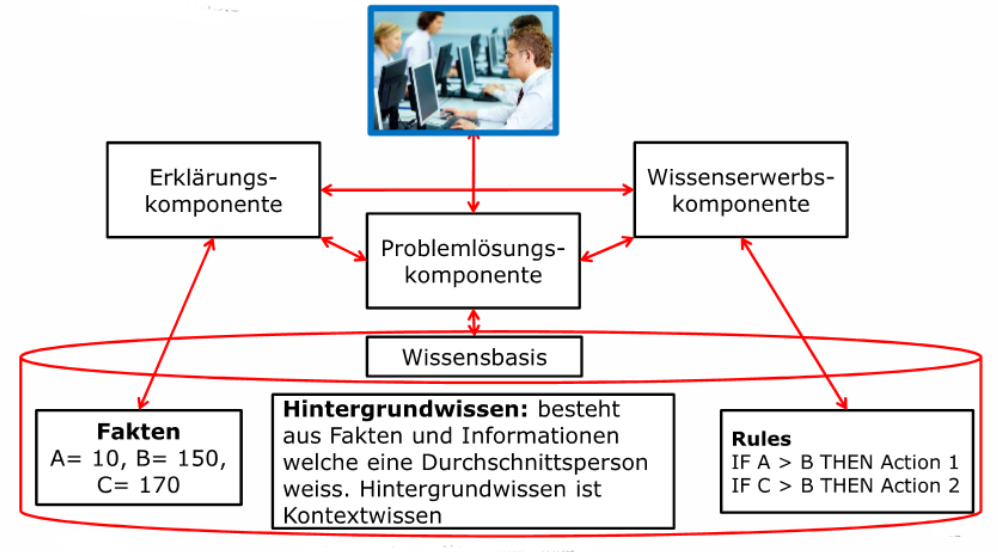
\includegraphics[keepaspectratio=true,height=15\baselineskip]{expertensystem.png}
	\caption{Beispiel eines Expertensystems}
	\label{fig:xps}
\end{figure}

\newpage

\subsection{Ungenügen der "gängigen" Datenhaltung (Skript S13)}

\begin{itemize}
	\item Verschiedene Datenformate
	\item Verschiedene Werkzeuge
	\item Heterogenität der Daten
		\subitem Technisch (Mainframe / DBMS / Flatfile etc)
		\subitem Logisch (Schemata / Formate / Darstellungen etc.)
		\subitem Syntaktisch (Datum / Codierung / Währung)
		\subitem Qualitativ (Fehlende / Falsche / Doppelte Werte)
		\subitem Verfügbarkeit (Permanent / Periodisch / Temporär)
		\subitem Rechtlich (Datenschutz / Zugriffsverwaltung / Archivierung)
\end{itemize}

$\longrightarrow$ Neuer Ansatz einer Datenaufbereitung muss her: \textbf{Homogenisierung}

\subsection{Ungenügen der operativen Datenbanken für Entscheide (Skript S13)}

"Reguläre" Datenbanken im Geschäftsumfeld sind zu fest mit geschäftsrelevanten Lese- und Schreiboperationen beschäftigt. Bei solchen Datenbanken spricht man von OLTP-System (Online Transactional Processing). Diese Datenbanken sind also ziemlich schlecht geeignet für eine analytische, vorausschauende Bewirtschaftung, da solche Auswertung viel Zeit und vor allem Rechen-Performance benötigen.

Ausserdem liegen Daten in OLTP-Datenbanken meist in der 3. Normalform vor. Während dies eine sehr vernetze und effiziente Art der Datenspeicherung ist, ist die 3. Normalform ein schlechtes Abbild des intuitiven Denkens eines Managers.

$\rightarrow$ Neuer Ansatz einer Datenbank muss her: \textbf{analytische Datenbanken}

\subsection{SQL-Abfragen für Management-Zwecke}
Zusätzlich zu den vorhin genannten Gründen, sind Manager des SQL meist nicht mächtig. Sie wollen lieben "Drag and Drop" Interfaces, um sich ihre Daten "zusammenzuklicken" wie z.b. Microsoft Access.

Zudem sind Datenbank-Abfragen stets \textbf{zweidimensional} in Tabellen dargestellt. Wenn man nun aber Daten in drei Dimensionen auswerten will (z.B. Zeit, Ort und Anzahl), so ist dies zwar möglich mittels Tabellen, aber nicht sonderlich leserfreundlich.

$\rightarrow$ Neuer Ansatz der Datenabfrage muss her: \textbf{OLAP}

\newgeometry{margin=0.5in}

\begin{landscape}
\subsection{OLAP vs OLTP}
	
	\centering
	
	\begin{tabular}[htbp]{|l|r|r|}
		\hline 
		Merkmal & OLTP System  & OLAP System  \\ 
		\hline 
		Ausrichtung auf & Programm, BWL Prozess & Mensch, Analyse\\ 
		\hline 
		Zeitliche Reichweite & Taktisch & Strategisch \\ 
		\hline 
		Entscheidungsstufe & Tief & Hoch \\ 
		\hline
		Zweck & Rationalisierung \& Automatisierung & Planung \& Entscheidung \\
		\hline
		Anwenderzahl &Hoch & Tief \\
		\hline
		Entscheidung & Deduktiv & Induktiv / Explorativ \\
		\hline
		Bewirtschaftung I & Ändernd & Befragend \\
		\hline
		Bewirtschaftung II & Auf Datensatzebene & Auf Aggregatsebene \\
		\hline
		Anwendungsmuster & Voraussehbar & Variierend \\
		\hline
		Befragungsmuster & Einfach & Komplex \\
		\hline
		Bearbeitung & Repetitiv & Ad hoc / unstrukturiert \\
		\hline
		Betriebliches Wissen & Verarbeitend & Generierend \\
		\hline
		Verteilungsgrad & Dezentral & Zentral \\
		\hline
		Performance-Bedarf & Durchgehend hoch & Variierend \\
		\hline
		Mehrbenutzersynchronisation & Hoch & Tief bis keine \\
		\hline
		Optimierung & Schneller Insert \& Delete & Schnelles Lesen \\
		\hline
		Transaktionsdurchsatz & Hoch & Tief \\
		\hline
		Transaktionsdauer & Kurte Mutationen weniger Tupel & Lange Abfragen vieler Tupel \\
		\hline
		Abfragen & Häufige, einfache Abfragen & Weniger häufige, komplexe Anfragen \\
		\hline
		Antwortzeiten & (Mili)sekunden & Sekunden, Minuten, Stunden \\
		\hline
		Endbenutzerwerkzeug-Hersteller & DB-Hersteller & Markt \\
		\hline
		Zeitbezug & Aktuell & Historisch \\ 
		\hline
		Zeitdimension & Zeitpunkt & Zeitraum \\
		\hline
		Beständigkeit & Dynamisch & Statisch \\
		\hline
		Granularität & Fein & Grob \\
		\hline
		Datenbestand & Vollständig & Lückenhaft \\
		\hline
		Redundanz & Normalisiert & Denormalisiert \\
		\hline
		Datenqualität / Aussagekraft & Tief & Hoch \\
		\hline
		Aufbereitung & Anwendungsneutral & Analyseorientiert \\
		\hline
		Aktualisierung & Laufend & Periodisch \\
		\hline
		Verarbeitungseinheit & Keon & Gross \\
		\hline
		Verteilungsgrad & Dezentral & Zentral \\
		\hline
		Datenquelle & Aktuelle Unternehmensdaten & Interne \& externe Daten \\
		\hline
	\end{tabular} 
	\end{landscape}

\restoregeometry

\section{Daten vs. Informationen vs. Wissen vs. Weisheit}

\begin{figure}[htb]
	\centering
	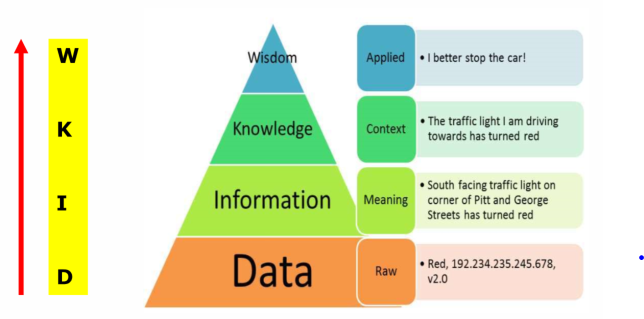
\includegraphics[keepaspectratio=true,height=15\baselineskip]{DIWW.PNG}
	\caption{DIKW-Pyramid}
	\label{fig:dikw}
\end{figure}

Bei Entscheidungsfindungen muss unterschieden werden zwischen

\begin{itemize}
	\item Daten
	\item Informationen
	\item Wissen
	\item Weisheit
\end{itemize}

\paragraph{Daten}
Daten sind das, was in Datenbanken oder Excel-Tabellen gespeichert wird. \textbf{Unstrukturierte Fakten} wie z.B die Zahlenreihenfolge 
\begin{center}
\textbf{	Rot, 192.234.235.245.678.v2.0}
\end{center}

\paragraph{Informationen}
Aus Daten alleine werden wir nicht schlau. Diese Daten müssen zuerst in einen \textbf{Zusammenhang} gebracht werden:

\begin{center}
\textbf{	Das südliche Rotlicht Pitt/George St. ist soeben rot geworden }
\end{center}

Nun können wir aus dieser, vorher völlig nutzlosen Zahlenreihe eine \textbf{Information} extrahieren. Nämlich dass sie Koordinaten sind und sich das "Rot" auf ein Lichtsignal bezieht..

Die Daten stellen zwar den eigentlichen Wert der Information dar (die Koordinaten und Rotlicht-Licht), sind aber ohne Zusammenhang völlig wertlos.

\paragraph{Wissen}
Aus Informationen \textbf{Wissen} zu machen ist nun, zumindest maschinell gesehen wesentlich schwerer. Wir Menschen generieren Wissen, indem wir Informationen geistig verarbeiten. Soll heissen, wir \textbf{interpretieren und ordnen} die gegebene Information.

Das heisst in diesem Fall, wir checken wo wir sind und in welche Richtung wir uns bewegen. Je nach dem ist das Wissen dann:

\begin{center}
\textbf{	Ich fahre in eine völlig andere Richtung, diese Information interessiert mich nicht.}
\end{center}

oder aber

\begin{center}
\textbf{	Das Rotlicht, auf welches ich zufahre, ist gerade rot geworden}
\end{center}

\paragraph{Weisheit}
Weisheit wird definiert als \textbf{Anwendung von Wissen auf eine Problemlösung}. Das heisst, das erworbene Wissen wird mit einer Portion Erfahrung und gesundem Menschenverstand gemixt. In unserem Fall, angenommen wir fahren auf das Rotlicht zu, sagt uns die Erfahrung, dass man bei einem roten Rotlicht stoppen soll und der gesunde Menschenverstand wirft noch ein, dass es entweder einen Unfall geben wird oder aber sicherlich eine Busse, sollte man erwischt werden. Das Ganze resultiert in:

\begin{center}
\textbf{	Ich sollte vermutlich nächstens einmal anhalten}
\end{center}

\vspace*{20px}

\begin{figure}[htb]
	\centering
	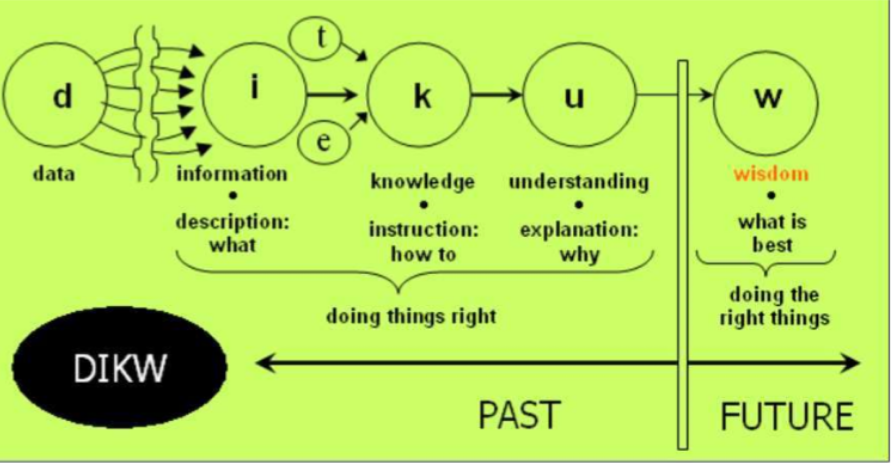
\includegraphics[keepaspectratio=true,height=15\baselineskip]{DIKW.PNG}
	\caption{Die Beziehung zwischen Daten - Informationen - Wissen - Weisheit}
	\label{fig:DIKW}
\end{figure}

Zusammengefasst kann man also sagen, Informationen sind das Verständnis von Zusammenhängen in Daten, oder auch \textbf{was die Daten bedeuten}. Wissen ist das Verständnis dieser Information (\textbf{was heisst das für mich?}) und Weisheit bestimmt, \textbf{was nun zu tun sei}. 
\newpage

\section{Das Data Warehouse}

\begin{wrapfigure}[10]{R}{0.5\textwidth}
	\centering
	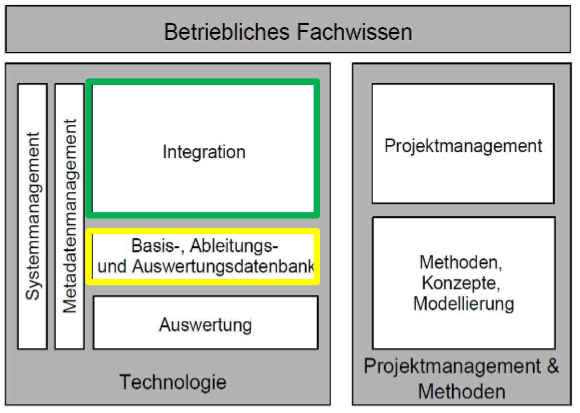
\includegraphics[keepaspectratio=true,height=10\baselineskip]{datawarehouse.PNG}
	\caption{Aufbau eines Datawarehouses}
	\label{fig:datawarehouse}
\end{wrapfigure}

In einer optimalen Welt würden Daten "perfekt" abgelegt werden, leicht zugänglich, platzsparend, sicher und für verschiedene Zwecke nützlich. Da wir aber leider nicht in einer optimalen Welt leben, ist dies nicht der Fall. (Buch S32)

Daten sind in der Praxis meist nicht optimal abgelegt. Daten existieren meist
\begin{itemize}
	\item in unterschiedlichen Formaten (Excel, Access, DB etc)
	\item in unterschiedlichen DB-Strukturen 
	\item in unterschiedlichen IT-Architekturen und -Systemen. Meist auch uralt Legacy-Systeme (Wie z.B. Cobol)
	\item zeit-aktuell und dynamisch
	\item zu detailliert und feingranular für wirksame Management-Abfragen
	\item in einem Format, das für Änderungstransaktionen optimiert wurde (z.B. 3. Normalform)
	\item mit begrenzten Zugriffsrechten (z.B. aus Security-Gründen)
	\item in einem schlecht verfügbaren Zustand (Legacy-System, proprietäres Format, Security-Gründe)
	\item in einem Format, welches komplexe SQL-Queries verlangt, um an Informationen oder Wissen zu gelangen.
\end{itemize}

$\rightarrow$ Lösung: \textbf{Data-Warehouse}

\newpage

\subsection{Definition Data-Warehouse (Skript S 33)}
	
\blockquote[Oracle corp: Data warehousing Guide 11g (2007)]{A data warehouse is a relational database that is designed for query and analysis rather than for transaction processing. It usually contains historic data derived from transaction data, but can incude data from other sources. Data warehouses separate analysis workload from transactin workload and enable an organisation to consoldiate data from several sources.} 
 

\blockquote[IBM Corp: Enterprise Data Warehousing with DB2.9 - Redbook (2008)]{A data warehouse is a organisation's data with a corporate wide scope for use in decision support and informational applications.}
\vspace*{10px}

Zusammengefasst kann man also sagen, ein Data Warehouse ist eine Datenbank, welche nicht (ausschliesslich) zur Speicherung von Informationen genutzt wird, sondern hauptsächlich als Hilfsmittel bei Entscheidungen eingesetzt wird ($\rightarrow$ Experten-Systeme)



\subsection{Bestandteile eines Data-Warehouses (Skript S39)}

\begin{description}
	\item [SSRS: ] SQL Server Reporting Services
	\item [SSAS: ] SQL Server Analysis Services
	\item [SSIS: ] SQL Server Integration Services
\end{description}

\begin{figure}[htb]
	\centering
	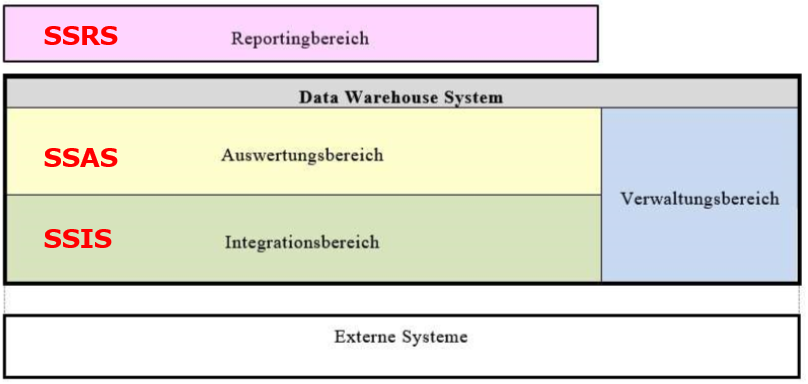
\includegraphics[keepaspectratio=true,height=15\baselineskip]{bestandteiledatawarehouse.PNG}
	\caption{Bestandteile eines Data-Warehouses}
	\label{fig:bstdw}
\end{figure}

\newpage

\subsection{Welche Datenbank für welche Tasks? (Buch S40f)}

\begin{figure}[htb]
	\centering
	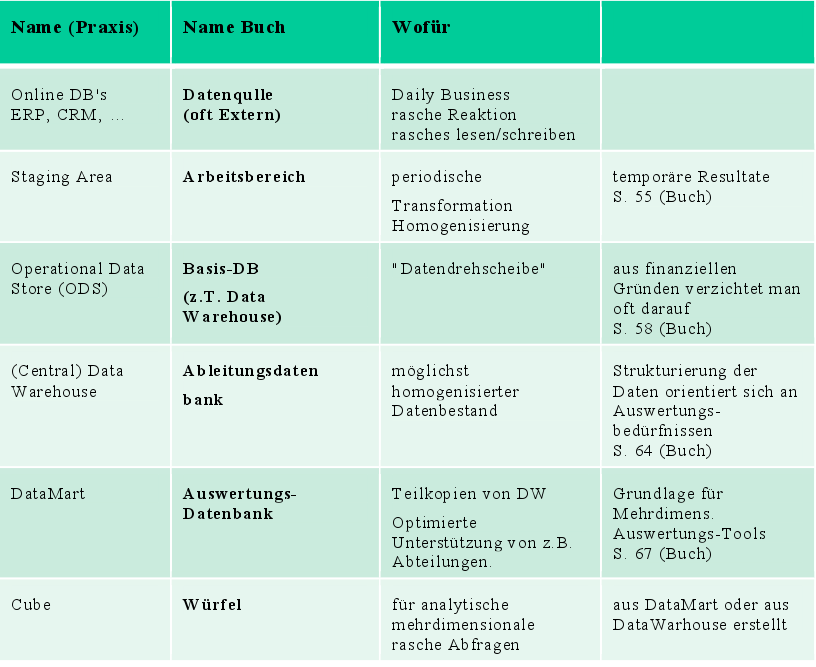
\includegraphics[keepaspectratio=true,height=18\baselineskip]{bestandteileDW.png}
	\caption{Welche Bestandteile eines Data-Warehouses werden für was benutzt?}
	\label{fig:bestDW}
\end{figure}


Verschiedene Datenbanken können (und sollten) für verschiedene Tasks verwendet werden.

\newpage

\section{Referenzarchitekturen}
\begin{wrapfigure}[15]{L}{0.5\textwidth}
	\centering
	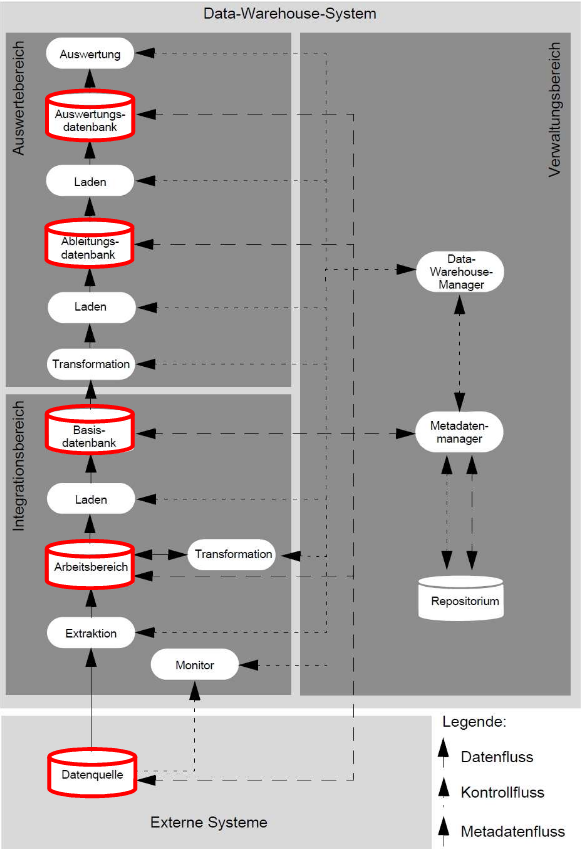
\includegraphics[keepaspectratio=true,height=18\baselineskip]{refModell.png}
	\caption{Referenzmodell eines Data Warehouses nach Bauer \& Günzel}
	\label{fig:refModel}
\end{wrapfigure}


Eine \textbf{Referenzarchitektur} ist ein Referenzmodell für eine Überklasse von Architekturen, in unserem Falle von Date Warehouses.

Ein \textbf{Referenzmodell} ist ein allgemeines Modell für eine Klasse von Dingen. Ein Referenzmodell sollte folgende zwei Eigenschaften haben:

\begin{itemize}
	\item Es können bestimmte Sachverhalte oder Modelle auf dessen Basis erstellt werden.
	\item Das allgemeine Modell kann als Vergleichsobjekt dienen.
\end{itemize}

In diesem Modul wird ausschliesslich mit dem hier dargestellten Referenzmodell von Bauer \& Günzel gearbeitet.

\vspace{3cm}

\subsection{Bestandteile des Referenzmodells (Skript S41)}
\subsubsection{Datenquelle}
Als \textbf{Datenquelle} eines Data-Warehouses werden oft beliebige\textit{ Bezugs-Datenbestände} benutzt (auch \textit{effektive Daten} oder \textit{Primärdaten} genannt)

Das können zum Beispiel:
\begin{itemize}
	\item Daten aus \textbf{Legacy-Systemen}
	\item Daten aus \textbf{Anwendungsprogrammen}
	\item Daten aus \textbf{zentralen/dezentralen Arbeitsplatz-DBs}
	\item \textbf{Textdateien} (z.B. im ASCII oder UTF-8 Format)
	\item Tabellen aus z.B Excel
\end{itemize}

sein.

\newpage

Es gibt weiterhin einige Probleme mit Datenquellen aus verschiedenen Systemen, wie zum Beispiel:
\begin{itemize}
	\item Unterschiedliche Zeichencodierung (ASCII, ANSI, UTF-8)
	\item Unterschiedliche Trennzeichen zwischen Datenfeldern (Komma, Semikolon)
	\item Unterschiedliche Zeilenwechsel (CR/LF, LF)
	\item Unterschiedlichen Sortierungen (alphanumerisch, numerisch)
\end{itemize}

Deshalb wird immer häufiger auf einheitliche XML-Inputs zurückgegriffen.

\subsubsection{Arbeitsbereich / Staging Area}
Der Arbeitsbereich integriert die Daten aus den verschiedenen vorhin genannten Datenquellen. Diese Integration passiert nach der Extraktion aus diesen Datenquellen.

Die Daten werden mit Hilfe des Metadaten-Repository anhand ihrer Metadaten zusammengefügt und abgelegt.

Das \textbf{Metadaten-Repository} besteht normalerweise aus verschiedenen Datenbank-Tabellen zur Verwaltung von Metadaten. Diese Metadaten stammen aus sehr unterschiedlichen Systemen und enthalten alle notwendigen Beschreibungen zu ihrem System und der Umwelt. Somit können die heterogenen Daten fast ohne Programmieraufwand zu einer homogenen Masse zusammengefügt werden.

\vspace{10px}

\noindent Die Staging Area ist ein \textbf{flüchtiges Zwischendepot} für die Daten. Hier werden die notwendigen Transformationen durchgeführt werden, welche in weiteren Schritten notwendig sind.

\subsubsection{Basis-DB / Operational Data Store (ODS)}
Ein ODS ist eine Datenbank, welche aktuelle/operative Daten hält, meist in kleinen Teilmengen unterteilt. Diese Datenbank ist eine \textbf{temporäre} Zwischenstation zwischen der Staging Area und dem Data Warehouse. 

\vspace{10px}

\noindent Das Datenmodell des OBS entspricht meist demjenigen der Datenquelle. Dies ist vor allem dann der Fall, wenn der OBS aus Leistungsgründen vom Quellsystem getrennt wurde und benutzt wird um gelegentliche Einzelfall-Analysen durchzuführen.

\vspace{10px}

\noindent Das Datenmodell des OBS kann andererseits auch demjenigen des Data Warehouses entsprechen. Dies ist dann der FAll, wenn der ODS als temporärer Zwischenspeicher zwischen den Quelldaten und dem Data Warehouse genutzt wird, oder aber wenn der ODS vom Data Warehouse Daten erhält.

Eine Basis-DB/ein ODS muss nach Gauer \& Günzel folgende Eigenschaften haben:
\begin{itemize}
	\item Die Daten sind \textbf{integriert} von den jeweiligen Datenquellen. Das heisst die verschiedenen Datenformate und Schematas wurden vereinheitlicht.
	\item Sie enthält nebst aktuellen Daten auch \textbf{historische Daten}, jedoch in geringerer Feingranularität wie das Data Warehouse.
	\item Sie ist \textbf{Anwendungsneutral}, d.h. sie ist nicht für eine spezielle Anwendung optimiert bzw. fokussiert.
	\item Nach einer definierten Zeitspanne werden die Daten in die \textbf{Ableitungsdatenbank} übertragen, wo sie je nach Auswertungsbedarf in einem anderen Detaillierungsgrad abgelegt werden.
	\item Die \textbf{Aktualisierung} der Daten erfolgt zu \textbf{beliebigen Zeitpunkten}. Dieser Zeitpunkt wird durch den Aktualisierungsbedarf gesteuert.
	\item Die Daten wurden bereits in der Staging Area bereinigt.
\end{itemize}

\vspace{10px}

\noindent Der ODS wird entweder laufend oder periodisch mit Daten aus der Staging Area gefüttert. Vor allem in kleineren Data Warehouse Systemen fällt der ODS sogar manchmal ganz weg und die Staging Area übernimmt auch diese Arbeiten. Im professionellen Umfeld sind jedoch sowohl der ODS wie auch die Stagin-Area ein integraler Bestandteil der Data Warehouse Architektur. 

\begin{figure}[htb]
	\centering
	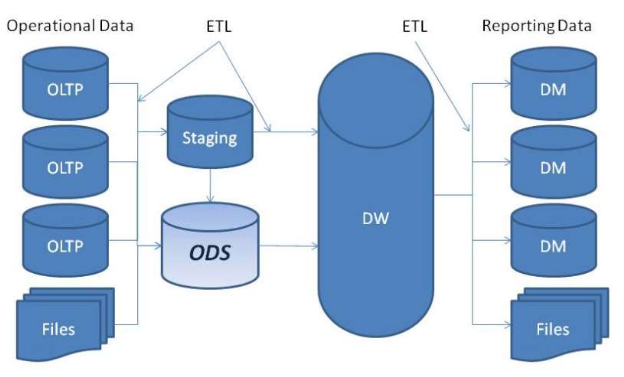
\includegraphics[keepaspectratio=true,height=15\baselineskip]{ODS.png}
	\caption{Eingliederung des ODS in die Data Warehouse Architektur}
	\label{fig:ODS}
\end{figure}

\subsubsection{Ableitungsdatenbank (=(Enterprise-)Data Warehouse)}
Wenn von einem Data Warehouse gesprochen wird, ist in der Regel ein \textit{Enterprise-Data-Warehouse} gemeint (= ein DWH mit unternehmensweitem Datenmodell und unternehmensweiten, universellen Datenbestand). 

\vspace{10px}

\noindent Die Datenbestände eines Data Warehouses werden zwar periodisch ergänzt, jedoch werden praktisch nie Daten gelöscht oder verändert, wenn sie mal im Data Warehouse sind. Aufgrund dessen beinhalten solche Systeme eine enorme Menge von Daten (auch VLDBs für Very Large DataBases).

Es ist jedoch selten nötig auf den gesamte§n Datenbestand dieser riesigen Datenbanken zuzugreifen. Aufgrund dessen werden Daten, die sehr selten benutzt werden in grossen Unternehmungen meist in Teilkopien des Data Warehouses, sogenannten \textit{Data Marts} gespeichert.

\subsubsection{Auswertungsdatenbank (Data-Mart)}
Ein Data-Mart ist eine \textbf{Teilkopie} eines Data-Warehouses, die aber auf demselben Datenmodell basieren. Solche Data-Marts werden meist für Abteilungen einer Unternehmung wie z.B. das Marketing erstellt. Der Vorteil dieser Data-Marts ist, dass diese unabhngig sind vom zentralen DW.

Vorteile eines Data-Marts sind z.B. 

\begin{itemize}
	\item Bessere Leistung, da nicht alle Analysen/Auswertungen auf dem zentralen DW gemacht werden müssen
	\item Entlastung des DW
	\item Im Falle von lokalen Data-Marts weniger Netzwerkbelastung
\end{itemize}

Die Pflege und (Weiter)Entwicklung des Data-Marts liegt jeweils in der Verantwortung der einzelnen Abteilungen.

\vspace{10px}

\noindent Dass ein Data-Mart existieren kann, \textbf{muss} ein zentrales Data-Warehouse existieren. Deshalb werden solche Data-Marts meist als \textbf{abhängige Data-Marts} bezeichnet.

 Diese abhängigen Data-Marts stehen im Gegensatz zu den (historischen) \textbf{unabhängigen Data-Marts}. Diese Data Mars erhalten ihre Daten direkt von verschiedenen Quellsystemen (gehen also nicht über ein zentrales Data-WArehouse). Jedoch widerspricht das dem Gedanken von einem zentralen "Datenhort" des Data-Warehousing und \textit{sollten} heute nicht mehr verwendet werden (oder man sollte sie zumindest nicht mehr als Data-Marts bezeichnen...)

Ein "Problem" von Data-Marts ist, dass sie unabhängig voneinander sind. Somit werden meist dieselben Aggregationen mehrmals auf verschiedenen Data-Marts durchgeführt, was auf längere Zeit nicht sehr kosteneffizient ist. Stattdessen sollten diese Aggregationen eher auf dem zentralen DW durchgeführt werden (was aber nicht immer geht, da die verschiedenen Abteilungen nicht wissen, dass diese Aggregation bereits in einem anderen Data-Mart durchgeführt wurde)

\begin{figure}[htb]
	\centering
	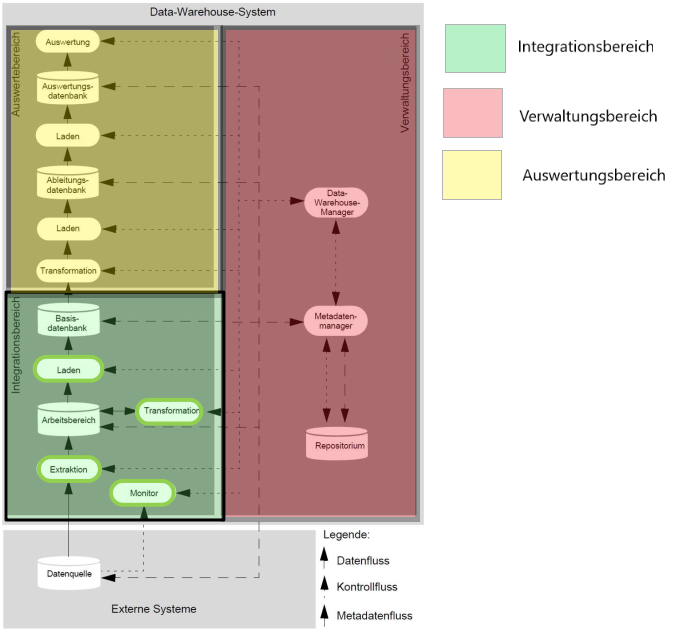
\includegraphics[keepaspectratio=true,height=18\baselineskip]{DWH_Bereiche.png}
	\caption{Bereiche eines Data-Warehouses nach Bauer \& Günzel}
	\label{fig:bereiche}
\end{figure}

\subsubsection{Integrationsbereich (Skript S51)}

Der Integrationsbereich bereitet die Daten, die aus verschiedenen Datenquellen kommen via staging area und ODS so auf, dass sie ins zentrale DW überführt werden können. 

Im Zusammenhang mit dem Integrationsbereich wird oft von \textbf{ETL} gesprochen. ETL steht für \textit{Extract - Transfer - Load} und entspricht den wesentlichen Arbeitsschritten, die durchgeführt werden müssen, bis die Daten vom Quellsystem im DW landen.

\subsubsection{Verwaltungsbereich}
%TODO
\subsubsection{Auswertungsbereich}
%TODO
\newpage

\subsection{Referenzmodelle in die Praxis umgesetzt (Skript S60)}
\subsubsection{"Hub and Spoke"-Architektur}
\begin{wrapfigure}[14]{L}{0.5\textwidth}
	\centering
	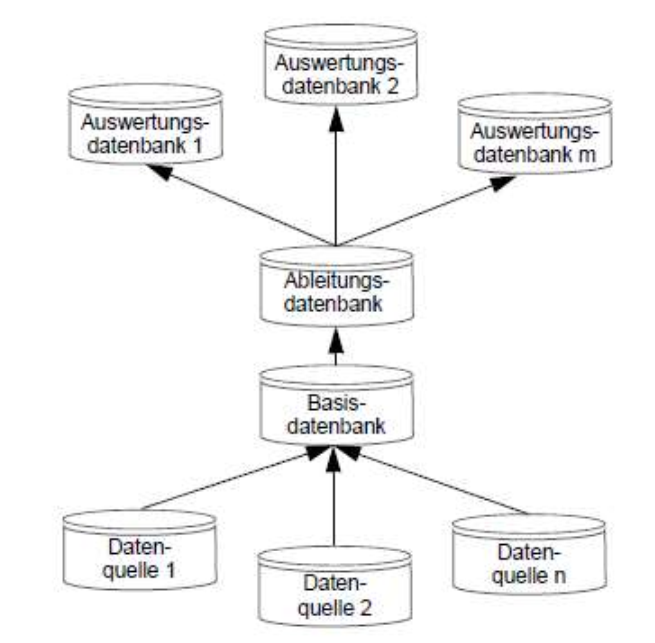
\includegraphics[keepaspectratio=true,height=16\baselineskip]{HubAndSpoke.PNG}
	\caption{Hub and Spoke / Nabe und Speiche Architektur}
	\label{label}
\end{wrapfigure}

Bei der Hub and Spoke (auch Nabe und Speiche Arhictektur) werden aus mehreren Quellsystemen (Speichen/Spokes) Daten in eine Basisdatenbank geladen, dort ETL-ed und anschliessend in eine Ableitungsdatenbank überführt (Hub/Nabe). Von dort werden sie anschliessend wieder in verschiedene Auswertung-Datenbanken verteilt (Speiche/Spokes).

\vspace{10px}

\noindent Das Core-Data-Warehouse ist also eine der zentralen Naben oder Hubs und ist verantwortlich für die Integration, QA und die Verteilung von Daten an die verschiedenen Data-Marts (Auswertungs-Datenbanken). 

\vspace{80px}


\subsubsection{Star-Architektur}

\begin{wrapfigure}[16]{R}{0.5\textwidth}
	\centering
	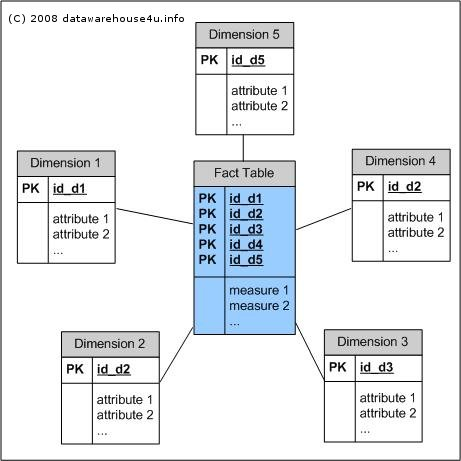
\includegraphics[keepaspectratio=true,height=16\baselineskip]{starschema.jpg}
	\caption{Starschema mit einer Fakttabelle in der Mitte und fünf Dimensionstabellen}
	\label{fig:star}
\end{wrapfigure}

Die Star- oder Stern-Architektur ist eine der drei am weitesten verbreiteten Datenmodelle. Sie besteht aus einer sog. \textbf{Faktentabelle} in der Mitte, die von mehreren \textbf{Dimensionstabellen} sternförmig umgeben ist. 

Durch eine solche Anordnung sind die Datenbanken normalerweise \textit{denormalisiert}, können also redundante Daten enthalten. Jedoch wird dieser eventuelle höhere Speicherbedarf in Kauf genommen, da ein solches Sternschema eine wesentliche höhere Performance bietet im ETL-Bereich wie eine normalisierte Datenbank.

\vspace{10px}

\noindent Eine weitere Verbesserung der Performance könnte man mit dem, aus der Stern-Architektur abgeleiteten \textbf{Schneeflockenarchitektur} erzielen.

\newpage

\subsubsection{Snowflake-Architektur}
\begin{wrapfigure}[21]{L}{0.7\textwidth}
	\centering
	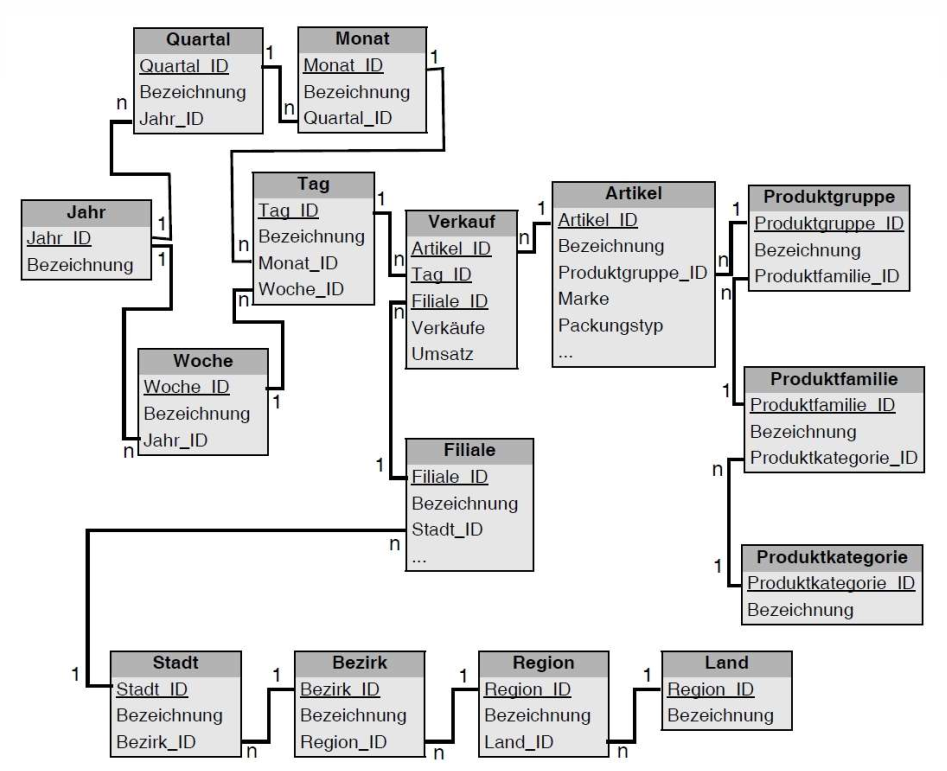
\includegraphics[keepaspectratio=true,height=18\baselineskip]{snowflake.PNG}
	\caption{Beispiel einer Schneeflocken-Architektur}
	\label{label}
\end{wrapfigure}

Die Snowflake- oder Schneeflocken-Architektur ist eng mit der Stenr-Architektur verbunden. Der einzige Unterschied zwischen der Stern- und der Schneeflocken-Architektur ist, dass die Dimensionstabellen gleichzeitig auch Faktentabellen sind, die wiederum von anderen Tabellen umgeben sind. Diese Dimensionstabellen werden über Joins verknüpft. 

\subsubsection{Galaxy-Architektur}

\begin{wrapfigure}[19]{R}{0.7\textwidth}
	\centering
	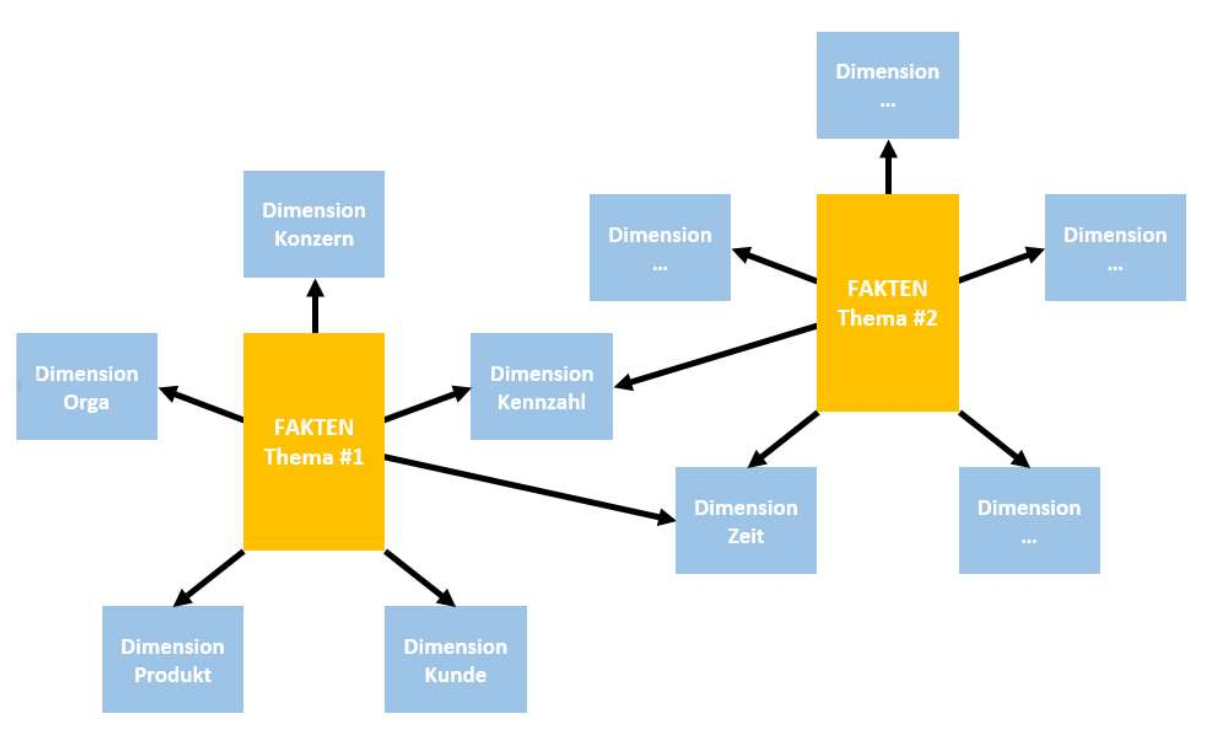
\includegraphics[keepaspectratio=true,height=15\baselineskip]{galaxy.PNG}
	\caption{Galaxy-Architektur}
	\label{fig:galaxy}
\end{wrapfigure}

Die Galaxy- oder Galaxie-Architektur ist ebenfalls stark mit dem Stern-Schema verwandt. Allerdings können sich hier mehrere Faktentabelle eine Dimensionstabelle teilen.

\vspace{20px}

\noindent Bei den drei oben genannten Architekturen werden Daten als \textbf{Fakten} bezeichnet und somit in der \textbf{Faktentabelle} gespeichert. Fakten werden, je nach Literatur auch \textbf{Metriken} oder \textbf{Kennzahlen} genannt. Solche Faktentabellen können über die Zeit sehr gross werden und enthalten Kennzahlen, die sich aus dem laufenden Geschäft ableiten lassen, wie z.B. Profitabilität, Kosten oder Ausgaben.

Wie in Abbildung \ref{fig:star} zu sehen ist, enthalten Faktentabellen Fremdschlüssel zu den Einträgen in den Dimensionstabellen. Das impliziert, dass es jeden Eintrag zu einer Kombination von Dimensionen nur einmal geben kann.

Im Gegensatz zu den riesigen und volatlen Faktentabellen sind Dimenstionstabellen recht statisch und vergleichsweise klein. 

\section{ETL}
\subsection{Extraktion}

Unter Extraktion versteht man die \textbf{Übertragung der Daten vom Quellsystem in die Staging Area}

\vspace{10px}

\noindent Je nach dem, welche Extraktions-Strategie gewählt wurde, werden die Daten zu unterschiedlichen Zeitpunkten extrahiert:

\begin{description}
	\item[Sofort] Der Extraktionsprozess wird bei jeder Änderung sofort gestartet
	\item[Trigger-/Ereignisbasiert] z.B. Beim Erreichen einer festgelegten Anzahl von Änderungen
	\item[Periodisch] Die Daten haben eine geforderte Mindestaktualität. Nach Ablauf dieser festgelegten Periode werden die Änderungen in eine sog. Snapshot-Datei überführt, die anschliessend in die Datenbank importiert wird.
	\item[Anfrage] Eine Anfrage auf die Datenbank erfordert aktualisierte Daten.
\end{description}

\vspace{10px}

\noindent Es gibt zwei grundsätzlich zwei \textbf{Extraktionstechniken}
\begin{description}
	\item[Replikationsbasiert] Geänderte Tupel werden in spezielle Tabellen geschrieben
	\item[Logbasiert] Jede Änderung wird in einer Logdatei protokolliert. Durch die Auswertung dieser Logdatei wird entschieden, welche Daten geändert und somit extrahiert werden müssen
\end{description}

\noindent Die Extraktion geschieht meist über SQL und es werden meist Schnittstellen zu den Datenbanken verwendet wie z.B. ODBC, OLE DB oder JDBC.

\vspace{10px}

\noindent \textbf{Open Database Connectivity (ODBC)} ist eine standardisierte Datenbankschnittstelle, mit welcher über SQL auf die Datenbank zugegriffen werden kann. Der Vorteil von ODBC ist, dass es eine API gibt, die es einem erlaubt, eine DB-Anwendung zu schreiben, die unabhängig vom Datenbankmanagement-System (DBMS) (mySQL, postgreSQL, Oracle etc) funktioniert, solange ODBC einen Treiber dafür hat.

\vspace{10px}

\noindent \textbf{Java Database Connectivity (JDBC)} ist eine universelle Java-basierte Datenbankschnittstelle für Datenbanken diverser Hersteller. JDBC ist vor allem auf relationale Datenbanken ausgelegt.


\subsection{Tranformation}

Nach der Extraktion müssen diese rohen Daten transformiert werden. Das heisst, sie müssen so aufbereitet werden, dass sie auch tatsächlich Sinn ergeben. Die Transformation lässt sich auf folgende Arbeitsschritte herunterbrechen:

\begin{description}
	\item[Data migration / Data wrangling] Daten werden \textbf{vereinheitlicht} also dass sie z.B. dieselben Masseinheiten oder Datenformate verwenden.
	\item[Data clean(s)ing] Daten werden \textbf{bereinigt}, also doppelte Daten gelöscht, falsche Daten korrigiert oder veraltete Daten aktualisiert.
\end{description}

\vspace{10px}

\noindent Dabei nimmt das Data Wrangling mit Abstand am meisten Zeit in Anspruch (bis zu 80\%)


\subsection{Load}

Die extrahierten und bereinigten Daten müssen nun noch in die \textbf{Basis- oder Ableitungsdatenbank übertragen} werden. Daür werden meist Ladewerkzeuge des Datenbankherstellers verwendet (SSIS bei SQL oder SQL*Loader bei Oracle)

\vspace{10px}

\noindent 
Weitere Möglichkeiten sind z.B. die SSIS Integration von Visual Studio, SSIS direkt oder DataWriter von IBM

\vspace{10px}

\textbf{SQL-Codebeispiele für den Load-Prozess}

\vspace{10px}

\noindent SQL-INSERT

\begin{lstlisting}[language=SQL]
INSERT INTO table_name
	VALUES (
		value1,
		value2,
		value3,
		...
	)
; 
\end{lstlisting}

\noindent SQL BULK INSERT

\begin{lstlisting}[language=SQL]
//FileType=1 (TxtFile1.txt)

"Kelly","Reynold","kelly@reynold.com" 
"John","Smith","bill@smith.com" 
"Sara","Parker", "sara@parker.com"

//FileType=2 (TxtFile2.txt) 

Kelly,Reynold,kelly@reynold.com 
John,Smith,bill@smith.com 
Sara,Parker,sara@parker.com 

BULK INSERT TmpStList FROM 'c:\TxtFile1.txt' WITH (FIELDTERMINATOR = '","') 
BULK INSERT tmpStList FROM 'c:\TxtFile2.txt' WITH (FIELDTERMINATOR = ',')
\end{lstlisting}


\vspace{10px}

\noindent Aufgrund dessen, dass während des Ladens die betroffenen Datenbanken gar nicht oder nur eingeschränkt nutzbar sind, ist die Effizienz des Ladevorgang essentiell. Aus diesem Grund werden Ladevorgänge meist in der Nacht, am frühen Morgen oder übers Wochenende durchgeführt.

Es wird dabei zwischen \textbf{Online- und Offline-Ladevorgängen} unterschieden. Beim Online-Laden kann die Datenbank weiterhin verwendet werden. Beim Offline-Ladevorgang ist die Datenbank während des Vorgangs offline, kann also nicht verwendet werden. Ob eine Datenbank einen Online-Ladevorgang unterstützt, hängt davon ab, ob die verwendete Anwendung oder Datenbank dies zur Verfügung stellt. So könnten z.B. während des Ladevorgang die Datenänderungen in ein Logfile geschrieben werden und dieses Logfile wird nach erfolgreichem Ladevorgang in die aktualisierte Datenbank übertragen.

Ebenfalls unterscheidet man zwischen dem \textbf{Initialisierungsladen} (alle Daten, DB wird zum ersten Mal gefüllt) und dem \textbf{Aktualisierungsladen} (nur geänderte Daten werden in die DB geladen)

Daten werden entweder in eine Basis- Ableitungs- oder Auswertungsdatenbank geladen. Aufgrund der grossen Datenmengen können nicht die normalen Datenmanipulationswerkzeuge eingesetzt werden. Stattdessen werden meist sog. \textbf{Bulk-Loader},die auf genau diese Tasks spezialisiert sind, verwendet. Diese Bulk-Loader verwenden aus Effizienzgründen keine Schnittstelle zur DB, sondern greifen direkt darauf zu. Deshalb können bestimmte Bulk-Loader auch nur für bestimmte Datenbanken verwendet werden. 

\subsection{Monitor}
Der Monitor spielt je nach Extraktionsstrategie eine wichtige Rolle. Er überwacht die Datenquellen und bemerkt somit Datenänderungen sofort. Je nach Extraktionsstrategie wird somit ein ETL-Prozess getriggert, ein Logeintrag oder eine Snapshot-Datei gemacht o.ä. 

Monitore haben vor allem in Data Warehouses eine sehr grosse Bedeutung. Dank ihnen müssen weniger DB-Zugriffe gemacht werden und gleichzeitig werden Redundanzen vermieden.

\vspace{10px}

\noindent Es gibt einige Sachen, die zu bedenken sind beim Einführen einer Monitor-Lösung:
\begin{itemize}
	\item Wird die gesamte Änderung festgehalten oder nur das neue/geänderte Tupel? ($\rightarrow$ Je nach dem Platzproblem)
	\item Benachricht das Quellsystem den Monitor sobald es eine Änderung gegeben hat ($\rightarrow$ Triggering) oder fragt der Monitor regelmässig beim Quellsystem nach ($\rightarrow$ Polling)? ($\rightarrow$ je nach dem, Überbelastung von Quell- oder Zielsystem)
	\item Überwacht das Quellsystem selbst, welche Änderungen erfolgen, oder wird dies von einem externen Dienst übernommen? ($\rightarrow$ Überbelastung Quellsystem vs. Kosten eines externen Dienstes)
	\item Sollen Änderungen sofort zum Data Warehouse gepusht werden oder nur zu bestimmten Zeiten (z.B. über Nacht)? ($\rightarrow$ Belastung des Data Warehouses und Quellsystems vs. Synchrone Daten.)
	
\end{itemize}

\section{Unstrukturierte Daten}
Ein Grossteil der Daten, der uns heute vorliegt, ist \textbf{unstrukturiert}. Das heisst, es ist mit viel Aufwand verbunden, aus grossen Datenmengen Informationen zu extrahieren (man denke z.B. daran, wie viel Aufwand es benötigen würde, um 10'000 E-Mails nach Thema zu sortieren vs. wie viel Aufwand es benötigt, 10'000 Datensätze nach ID zu sortieren).

Mithilfe von \textbf{strukturierten Daten} kann man \textit{automatisiert} Informationen aus Datenquellen extrahieren und aufbereiten.

\subsection{Nutzen}

\noindent Wenn man heute unstrukturierte Daten auswerten würde, könnte man z.B. automatisch Kundenbewertungen und -beschwerden aus Foren und Blogs auslesen, Twitter-Posts analysieren u.v.m. 

Zusammengefasst kann man sagen: Unstrukturierte Daten ermöglichen \textbf{Analysen, die zu schnellen Reaktionen und Entscheidungen führen}.

\newpage

\subsection{Herausforderungen}

\begin{itemize}
	\item Kein vorgegebenes/einheitliches Schema
	\item Kein vorgegebenes/einheitliches Datenformat
	\item Semantikabhängig (z.B. JSON vs. XML)
	\item Grosse Mengen $\rightarrow$ können nicht manuell ausgewertet werden.
	\item Priorität kann nicht automatisiert gemessen werden.
	\item Datenqualität kann nicht automatisiert gemessen werden
\end{itemize}

\subsection{Analyse}

\subsubsection{NLP - Natural Language Processing (Skript S70)}
 NLP beschreibt die Techniken und Methoden zur maschinellen Verarbeitung natürlicher Sprache. Ziel ist eine direkte Kommunikation zwische nMensch und coputer auf Basis der natürlichen (menschlichen) Sprache.

NLP ist eine sehr AI-lastige Technologie und mittels welcher Text in strukturierte Informationen gebündelt werden kann. NLP setzt sich mittels der Verarbeitung der natürlichen Sprache, dem Verstehen und der Semantik von 
Wörtern und Sätzen der Klassifizierung von Texten auseinander.

\subsubsection{Data Mining}
 Data Mining ist die systematische Anwendung statistischer Methoden auf grosse Datenbestände mit dem Ziel, neue Querverbindungen und Trends zu erkennen.

\subsubsection{Text Mining}
 Text Mining ist eine Untermethode von Data Mining und konzentriert sich vor allem auf Data Mining von grossen Texten wie z.B. die Plagiaterkennung, die gesamte Doktorarbeiten durchliest und analysiert.
 
 \subsubsection{Klassifikation}
 Klassifikation versucht, den Datenbestand in vorgegebene Klassen zuzuordnen.
 
 \newpage
 
 \subsubsection{Clustering}
 
  \begin{figure}[htb]
 	\centering
 	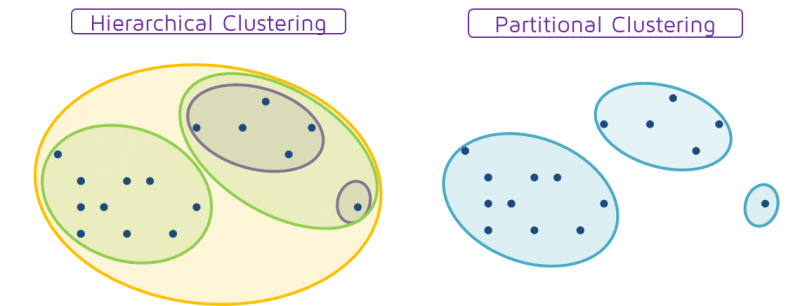
\includegraphics[keepaspectratio=true,height=12\baselineskip]{clustering.png}
 	\caption{Partitionierendes vs. Hierarchisches Clustering}
 	\label{fig:Clustering}
 \end{figure}
 
 Clustering ist ähnlich wie die Klassifikation, allerdings werden beim Clustering-Verfahren automatisch passende Klassen erstellt. Das Clustering-Verfahren zielt darauf ab, Gruppen oder Klassen zu erstellen, innerhalb von welchen sich die Objekte sehr ähnlich sind. Gleichzeitig sollten sich die erstellten Gruppen aber möglichst stark voneinander unterscheiden.
 
 Clustering wird normalerweise nur zu Beginn ausgeführt, um Klassen zu erstellen, mit welchen anschliessend eine Klassifikation durchgeführt werden kann.
 
 \vspace{10px}
 
 \noindent Es wird generell zwischen dem \textbf{partitionierenden} Clustering und dem \textbf{hierarchischen} Clustering unterschieden (Abbildung \ref{fig:Clustering}):
 
 \paragraph{Partitionierendes Clustering} unterteilt die gegebenen Daten in eine \textbf{vorgegebene Anzahl} von Klassen. Dabei werden zuerst die vorgebene Anzahl Clusterzentren/Klassen aus den Datensätzen ausgewählt. Anschliessend werden die restlichen Datensätze diesen Clusterzentren zugeordnet. 
 
 Nach dem ersten Durchgang werden erneut Clusterzentren/Klassen gewählt und die Daten werden wiederum diesen, neuen, Clusterzentren zugeordnet. Dieses ganze Spiel wird solange wiederholt, bis die Daten 'optimal' geclustert sind (möglichst ähnlich innerhalb der Klasse/des Clusters, möglichst verschieden zwischen den Klassen/Cluster).
 
   \begin{figure}[htb]
 	\centering
 	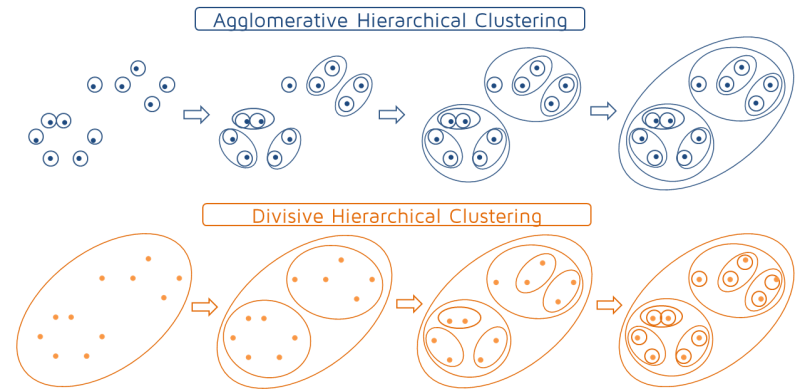
\includegraphics[keepaspectratio=true,height=12\baselineskip]{hierarchical_clustering.png}
 	\caption{Beispiel von agglomerativem (oben) und diversiven (unten) clustering}
 	\label{fig:hierCluster}
 \end{figure}
 
 \paragraph{Hierarchisches Clusteriong} kann wiederum in \textit{agglomeratives} und \textit{diversives} Clustering unterteilt werden. (Siehe Abbildung \ref{fig:hierCluster})
 
 Das \textit{agglomerative} Clustering funktioniert so, dass jeder Datensatz eine eigene Klasse/ein eigenes Cluster ist. Anschliessend werden die \textbf{zwei ähnlichsten Klassen zu einer zusammengefasst}. Dieses Zusammenfassen zweier ähnlicher Klassen wird solange durchgeführt wird, bis alle Daten in einem einzigen Cluster zusammengeführt sind.
 
 \vspace{10px}
 
 \noindent Beim \textit{diversiven} Clustering geht es in die andere Richtung. Die Datensätze werden bei jeder Iteration so halbiert, dass die Elemente innerhalb eines Clusters sich so ähnlich wie möglich sind, die Cluster untereinander aber möglichst unterschiedlich zueinander sind ('optimale' Cluster also). Diese Unterteilung wird solange fortgesetzt, bis jeder Datensatz seinen eigenen Cluster hat. Dieses Verfahren wird in der Praxis aber eher weniger angewandt.
 
 \subsubsection{Visualisierungstechnik}
 \begin{wrapfigure}[10]{L}{0.6\textwidth}
 	\centering
 	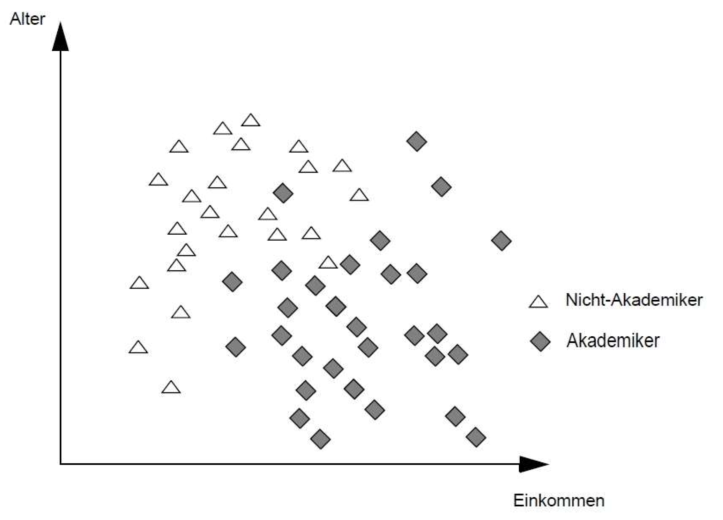
\includegraphics[keepaspectratio=true,height=13\baselineskip]{streudiagramm.PNG}
 	\caption{Daten visuell aufbereitet mittels eines Streudiagrammes}
 	\label{fig:streu}
 \end{wrapfigure}
 Bei der Visualisierungstechnik überlässt man die tatsächliche Auswertung dem Menschen. Die Daten werden mittels \textbf{zwei bis drei Merkmalen} im \textbf{zwei- oder dreidimensionalen} Raum dargestellt (z.B. Streudiagramm, siehe Abbildung \ref{fig:streu}). Es ist nun dem Menschen überlassen, aus dieser Grafik etwas nützliches herauszulesen.
 
 \vspace{90px}

\subsubsection{Fallbasierte Systeme}

\begin{wrapfigure}[12]{R}{0.5\textwidth}
	\centering
	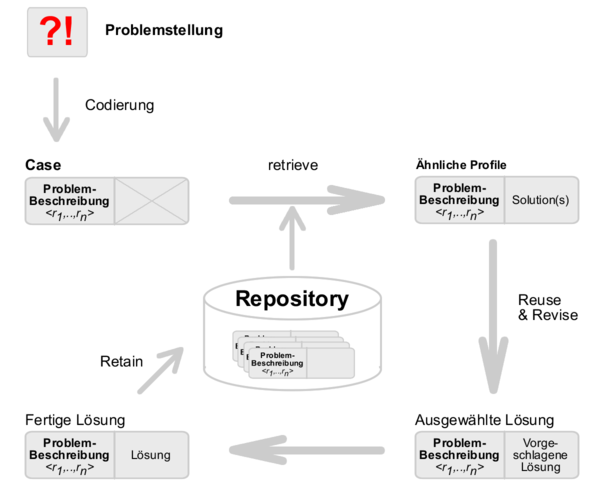
\includegraphics[keepaspectratio=true,height=12\baselineskip]{fallbasiert.png}
	\caption{Funktionsweise eines Fallbasierten Systemes}
	\label{fig:fallbasiert}
\end{wrapfigure}

Solche Systeme greifen auf Daten von ähnlichen, bereits gelösten Problemen zurück. Es gibt eine \textbf{Falldatenbank} gefüllt mit bereits gelösten, getaggeden oder anderswie codierten Problemen, auf welche zugegriffen werden kann. (Siehe Abbildung \ref{fig:fallbasiert})

Dieses System beruht auf der Annahme, dass geringe Änderungen an einer Problemstellung auch nur geringe Änderungen am Lösungsweg zur Konsequenz habenn (also \textbf{lineare Probleme}). Somit sind fallbasierte Systeme \textit{nicht} geeignet, um komplexe Probleme zu lösen.

\newpage

\subsubsection{Entscheidungsbaumverfahren (Buch S136)}
Ein Entscheidungsbaum ist die \textbf{grafische Darstellung einer Datenteilung} (z.B. mittels Clustering). Dabei stellen die nicht-Blatt Knoten des Baumes die Merkmale der Daten dar, nach denen der Datensatz geteilt wird. Über die Kanten werden diese Merkmale verbunden. Die Teildatenbestände (z.B. Cluster oder Klassen) werden schlussendlich in den Blättern dargestellt.

\vspace{10px}

\noindent Ein solcher Baum wird mittels des \textbf{Entscheidu9ngsbaumverfahrens}. Zuerst wird ein Merkmal bestimmt, nach welchem sortiert werden soll (in Abbildung \ref{fig:tree} wäre dies z.B. ob \\ 
$Schalengewicht <= 0.168$ und  $MSE = 10.273$ ist) und es wird danach sortiert. Dieser Vorgang wird nun wiederholt (dieses mal ist z.B. das Merkmal links $Schalengewicht <=0.059$ und $MSE = 4.635$ ist).

Der Vorgang wird nun solange wiederholt, bis alle Datensätze zu einem Cluster gehören, oder sich kein Merkmal mehr finden lässt, durch welches geteilt werden kann.

\begin{figure}[htb]
	\centering
	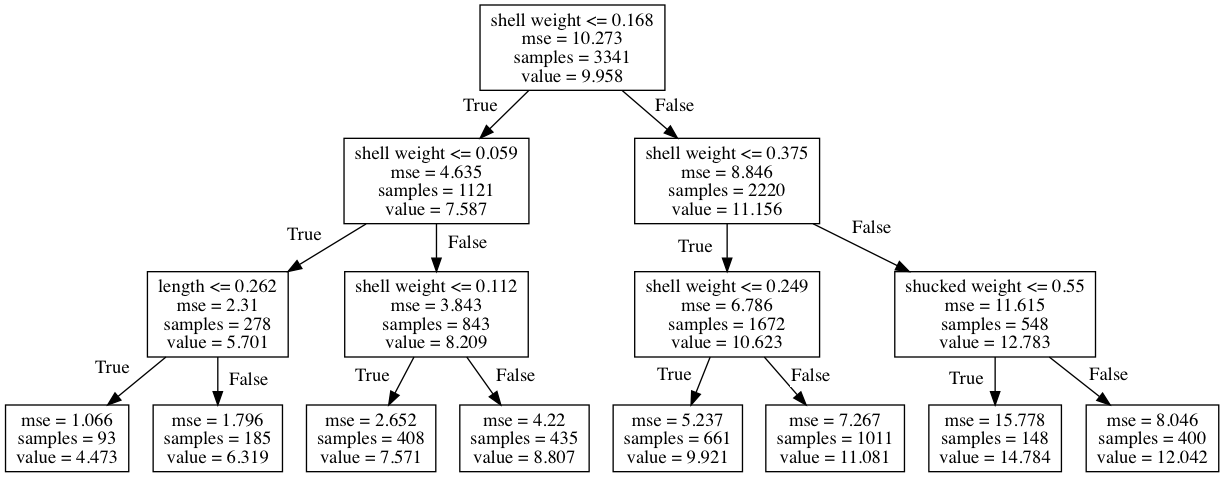
\includegraphics[keepaspectratio=true,height=13\baselineskip]{tree.png}
	\caption{Beispiel eines Entscheidungsbaumes}
	\label{fig:tree}
\end{figure}

Um Bäume zu verbessern, die eine hohe Fehlerquote aufweisen, kann \textbf{Pruning} verwendet werden. Dabei werden einzelne Knoten und Kanten des Baumes entfernt, um den Baum zu verkleinern und somit die Teilgenauigkeit des Baumes insgesamt zu erhöhen.

\vspace{10px}

\noindent Entscheidungsbäume werden zum Beispiel zur \textbf{Klassifizierung} von Daten hinzugezogen werden, um die Klassen einfacher und übersichtlicher darstellen zu können.


\end{document}
